% =============================================================================
% IEEE conference paper skeleton (IEEEtran). Compile with pdflatex + bibtex.
% Tables are generated by the pipeline: \input the .tex files in results/tables/.
% Figures are in results/figures, results/roc_curves, results/confusion_matrices.
% Replace [bracketed] text and fill numbers from results/metrics/*.json (or paste
% the rendered values from reports/thesis_rendered.md). DO NOT hard-code unverified
% numbers.
% =============================================================================
\documentclass[conference]{IEEEtran}
\usepackage{cite,graphicx,booktabs,amsmath}
\graphicspath{{../results/figures/}{../results/roc_curves/}{../results/confusion_matrices/}}

\begin{document}

\title{Memory-Efficient Explainable Pneumonia Detection Using Quantized
EfficientNet-B0 for Resource-Constrained Healthcare Environments}

\author{\IEEEauthorblockN{Rohan Maleku}
\IEEEauthorblockA{[Department]\\ [University]\\ rohan.maleku@gmail.com}}

\maketitle

\begin{abstract}
Pneumonia screening from chest X-rays is valuable in low-resource settings, but
high-capacity models are heavy and opaque. We present a reproducible framework
combining a lightweight EfficientNet-B0 backbone, integrated Grad-CAM++
explanations, and post-training INT8 quantization (dynamic and static PTQ), with
rigorous statistical and efficiency reporting. Against ResNet-18 and
MobileNetV3-Small baselines under an identical pipeline, we report test ROC-AUC,
sensitivity, and specificity with bootstrap 95\% confidence intervals, and quantify
the size/latency/accuracy trade-off of quantization. [State 1--2 headline measured
results once rendered.] All code, configs, and artifacts are released; no results
are simulated.
\end{abstract}

\begin{IEEEkeywords}
pneumonia detection, chest X-ray, EfficientNet, Grad-CAM++, quantization, edge AI,
explainable AI, reproducible research
\end{IEEEkeywords}

\section{Introduction}
[Motivation: pneumonia burden; need for deployable, transparent screening.
Contributions: (1) integrated reproducible framework; (2) correct efficiency
benchmarking; (3) transparent dynamic-vs-static quantization study; (4) open,
non-fabricated artifacts.]

\section{Related Work}
[CXR deep learning (CheXNet)~\cite{rajpurkar2017}; lightweight CNNs
(EfficientNet~\cite{tan2019}); XAI (Grad-CAM++~\cite{chattopadhay2018}); PTQ and
edge deployment. Identify the integration/reproducibility gap.]

\section{Methodology}
\subsection{Dataset and Splits}
Kermany pediatric CXR~\cite{kermany2018}; stratified validation split from train,
official test held out; automated duplicate and leakage checks. See Table~\ref{tab:dataset}.
\begin{table}
\caption{Dataset Statistics}
\label{tab:dataset}
\begin{tabular}{lrrrr}
\toprule
Split & Normal & Pneumonia & Total & Pneumonia ratio \\
\midrule
train & 1073 & 3099 & 4172 & 0.742800 \\
val & 268 & 776 & 1044 & 0.743300 \\
test & 234 & 390 & 624 & 0.625000 \\
total & 1575 & 4265 & 5840 & 0.730300 \\
\bottomrule
\end{tabular}
\end{table}


\subsection{Model and Training}
EfficientNet-B0 backbone with a shared binary head; staged freeze/unfreeze transfer
learning; AdamW, warmup+cosine schedule, label smoothing, AMP, early stopping.
Identical pipeline for ResNet-18 and MobileNetV3-Small. See Table~\ref{tab:trainconfig}.
\begin{table}
\caption{Training Configuration}
\label{tab:trainconfig}
\begin{tabular}{ll}
\toprule
Hyperparameter & Value \\
\midrule
Backbone & efficientnet\_b0 \\
Pretrained & ImageNet \\
Image size & 224x224 \\
Batch size & 32 \\
Optimizer & AdamW \\
Learning rate & 0.000300 \\
Weight decay & 0.000100 \\
LR schedule & 3-epoch warmup + cosine \\
Epochs & 20 \\
Unfreeze epoch & 8 \\
Label smoothing & 0.050000 \\
Early stopping patience & 7 \\
Gradient clipping & 1.000000 \\
Mixed precision & True \\
Seed & 42 \\
\bottomrule
\end{tabular}
\end{table}


\subsection{Evaluation, Explainability, Quantization, Benchmarking}
Bootstrap 95\% CIs for accuracy/AUC; Youden-J threshold; Grad-CAM++ for
correct/FP/FN cases; dynamic and static INT8 PTQ; correct latency/throughput/size
and sampled peak-RSS benchmarking (no \texttt{tracemalloc}).

\section{Results}
\subsection{Diagnostic Performance and Baselines}
\begin{table}
\caption{Final Test Performance}
\label{tab:final}
\begin{tabular}{lrl}
\toprule
Metric & Value & 95\% CI \\
\midrule
ROC-AUC & 0.967800 & [0.9504, 0.9816] \\
Accuracy & 0.918300 & [0.8958, 0.9391] \\
Sensitivity (Recall) & 0.966700 & — \\
Specificity & 0.837600 & — \\
Precision & 0.908400 & — \\
F1-score & 0.936600 & — \\
\bottomrule
\end{tabular}
\end{table}

\begin{table}
\caption{Model Comparison}
\label{tab:models}
\begin{tabular}{lrrrrrrrr}
\toprule
Model & Params (M) & AUC & Accuracy & Sensitivity & Specificity & F1 & Latency (ms) & Size (MB) \\
\midrule
efficientnet\_b0 & 4.340000 & 0.967800 & 0.918300 & 0.966700 & 0.837600 & 0.936600 & 164.050000 & 17.661000 \\
resnet18 & 11.310000 & 0.959400 & 0.879800 & 0.992300 & 0.692300 & 0.911700 & 103.525000 & 45.321000 \\
mobilenetv3\_small & 1.080000 & 0.974300 & 0.875000 & 0.997400 & 0.670900 & 0.908900 & 76.812000 & 4.442000 \\
\bottomrule
\end{tabular}
\end{table}


\begin{figure}[t]\centering
  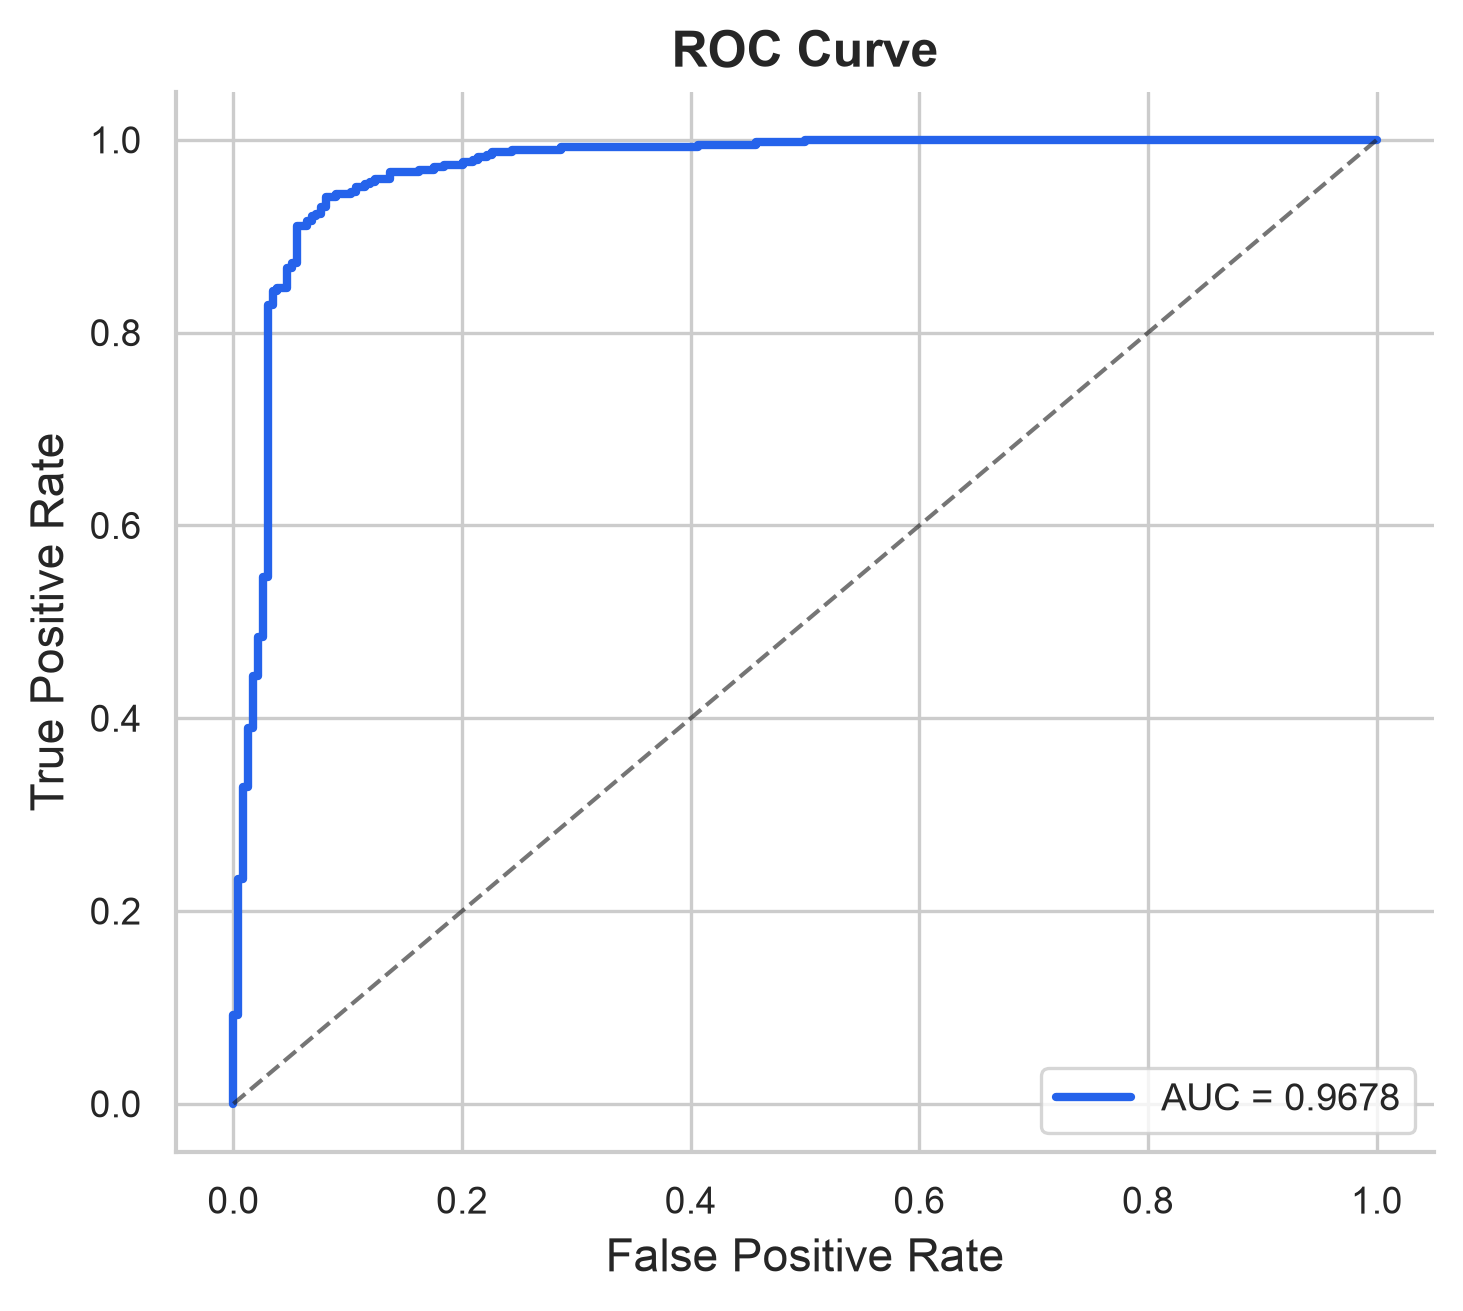
\includegraphics[width=\columnwidth]{efficientnet_b0_roc_curve.png}
  \caption{ROC curve on the held-out test set.}\label{fig:roc}
\end{figure}

\subsection{Quantization and Efficiency}
\begin{table}
\caption{Quantization Results (backend: qnnpack)}
\label{tab:quant}
\begin{tabular}{lrrrrrrr}
\toprule
Variant & Size (MB) & Size ↓ (\%) & Accuracy & Acc drop (\%) & AUC & AUC drop (\%) & Latency (ms) \\
\midrule
FP32 & 17.667000 & 0.000000 & 0.918300 & 0.000000 & 0.967800 & 0.000000 & 133.407000 \\
INT8 dynamic & 16.688000 & 5.500000 & 0.919900 & -0.160000 & 0.968200 & -0.040000 & 135.504000 \\
INT8 static (PTQ) & 5.219000 & 70.500000 & 0.810900 & 10.740000 & 0.944400 & 2.340000 & 16.294000 \\
\bottomrule
\end{tabular}
\end{table}

\begin{table}
\caption{Computational Efficiency}
\label{tab:efficiency}
\begin{tabular}{lrrrrr}
\toprule
Variant & Size (MB) & Latency mean (ms) & Latency p95 (ms) & Throughput (img/s) & Peak RSS Δ (MB) \\
\midrule
efficientnet\_b0\_fp32 & 17.661000 & 119.698000 & 120.615000 & 18.970000 & 314.770000 \\
\bottomrule
\end{tabular}
\end{table}


\begin{figure}[t]\centering
  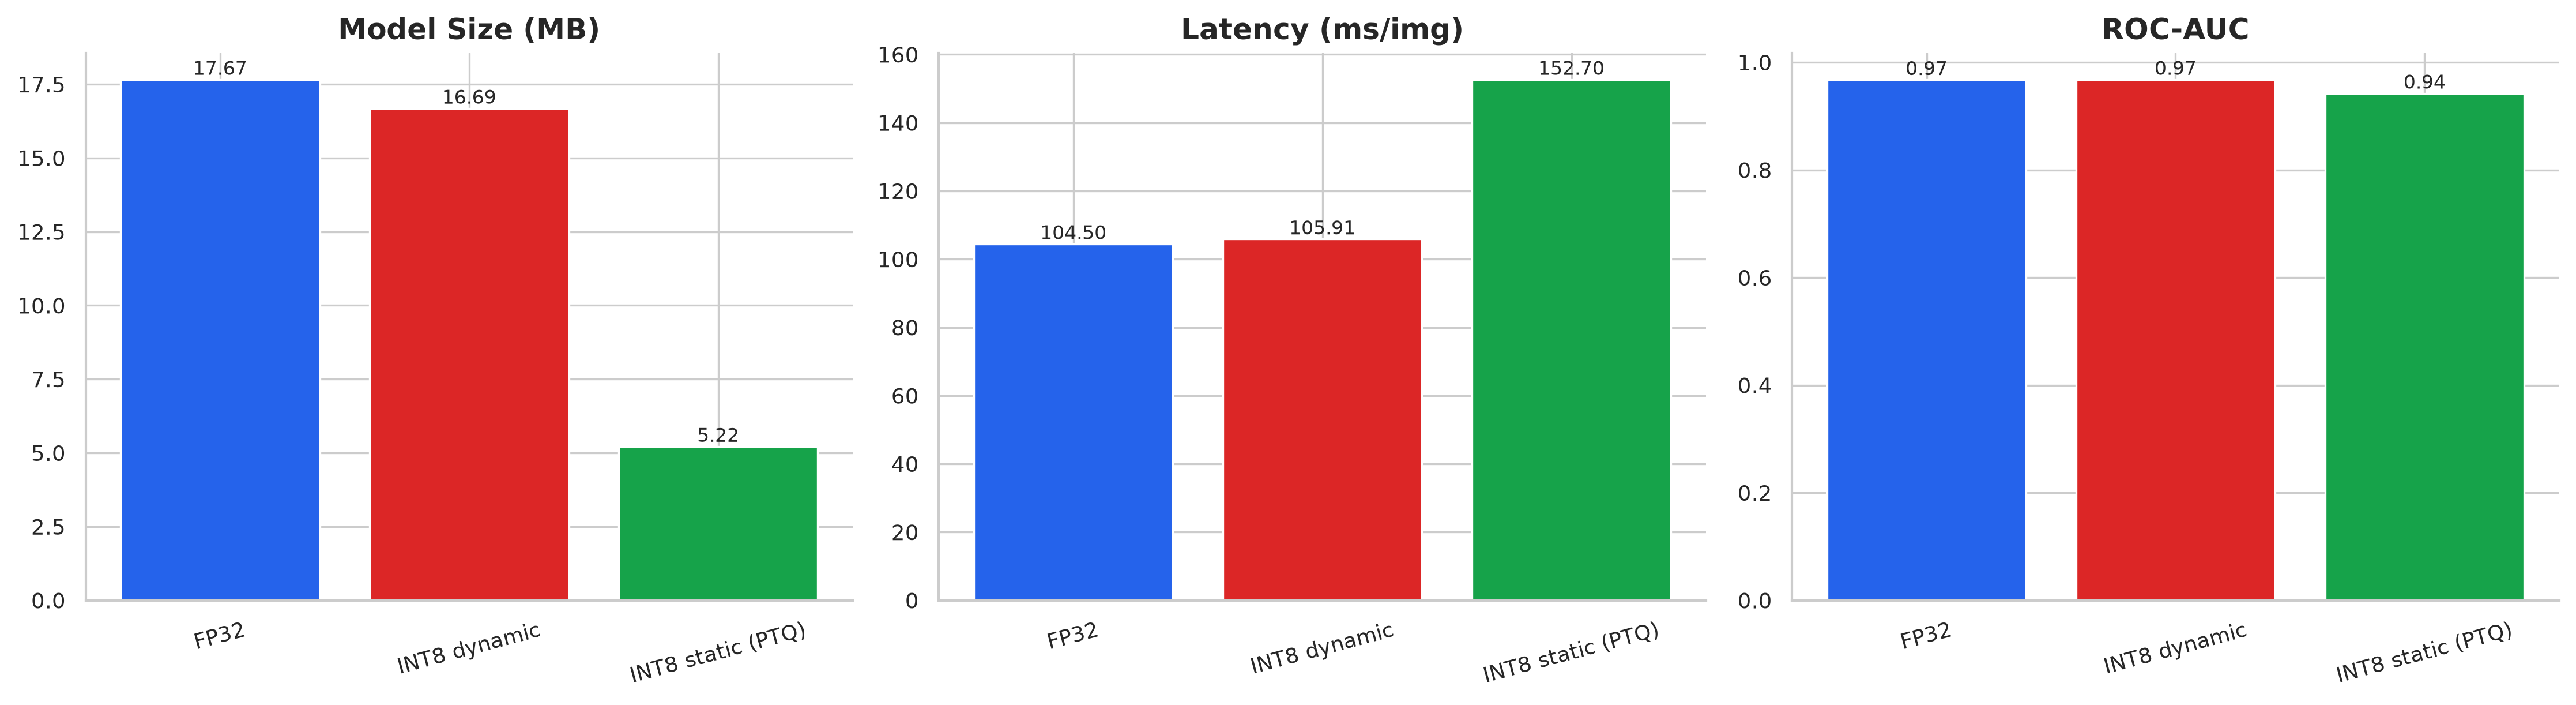
\includegraphics[width=\columnwidth]{quantization_comparison.png}
  \caption{FP32 vs INT8 (dynamic/static): size, latency, AUC.}\label{fig:quant}
\end{figure}

\subsection{Explainability}
\begin{figure}[t]\centering
  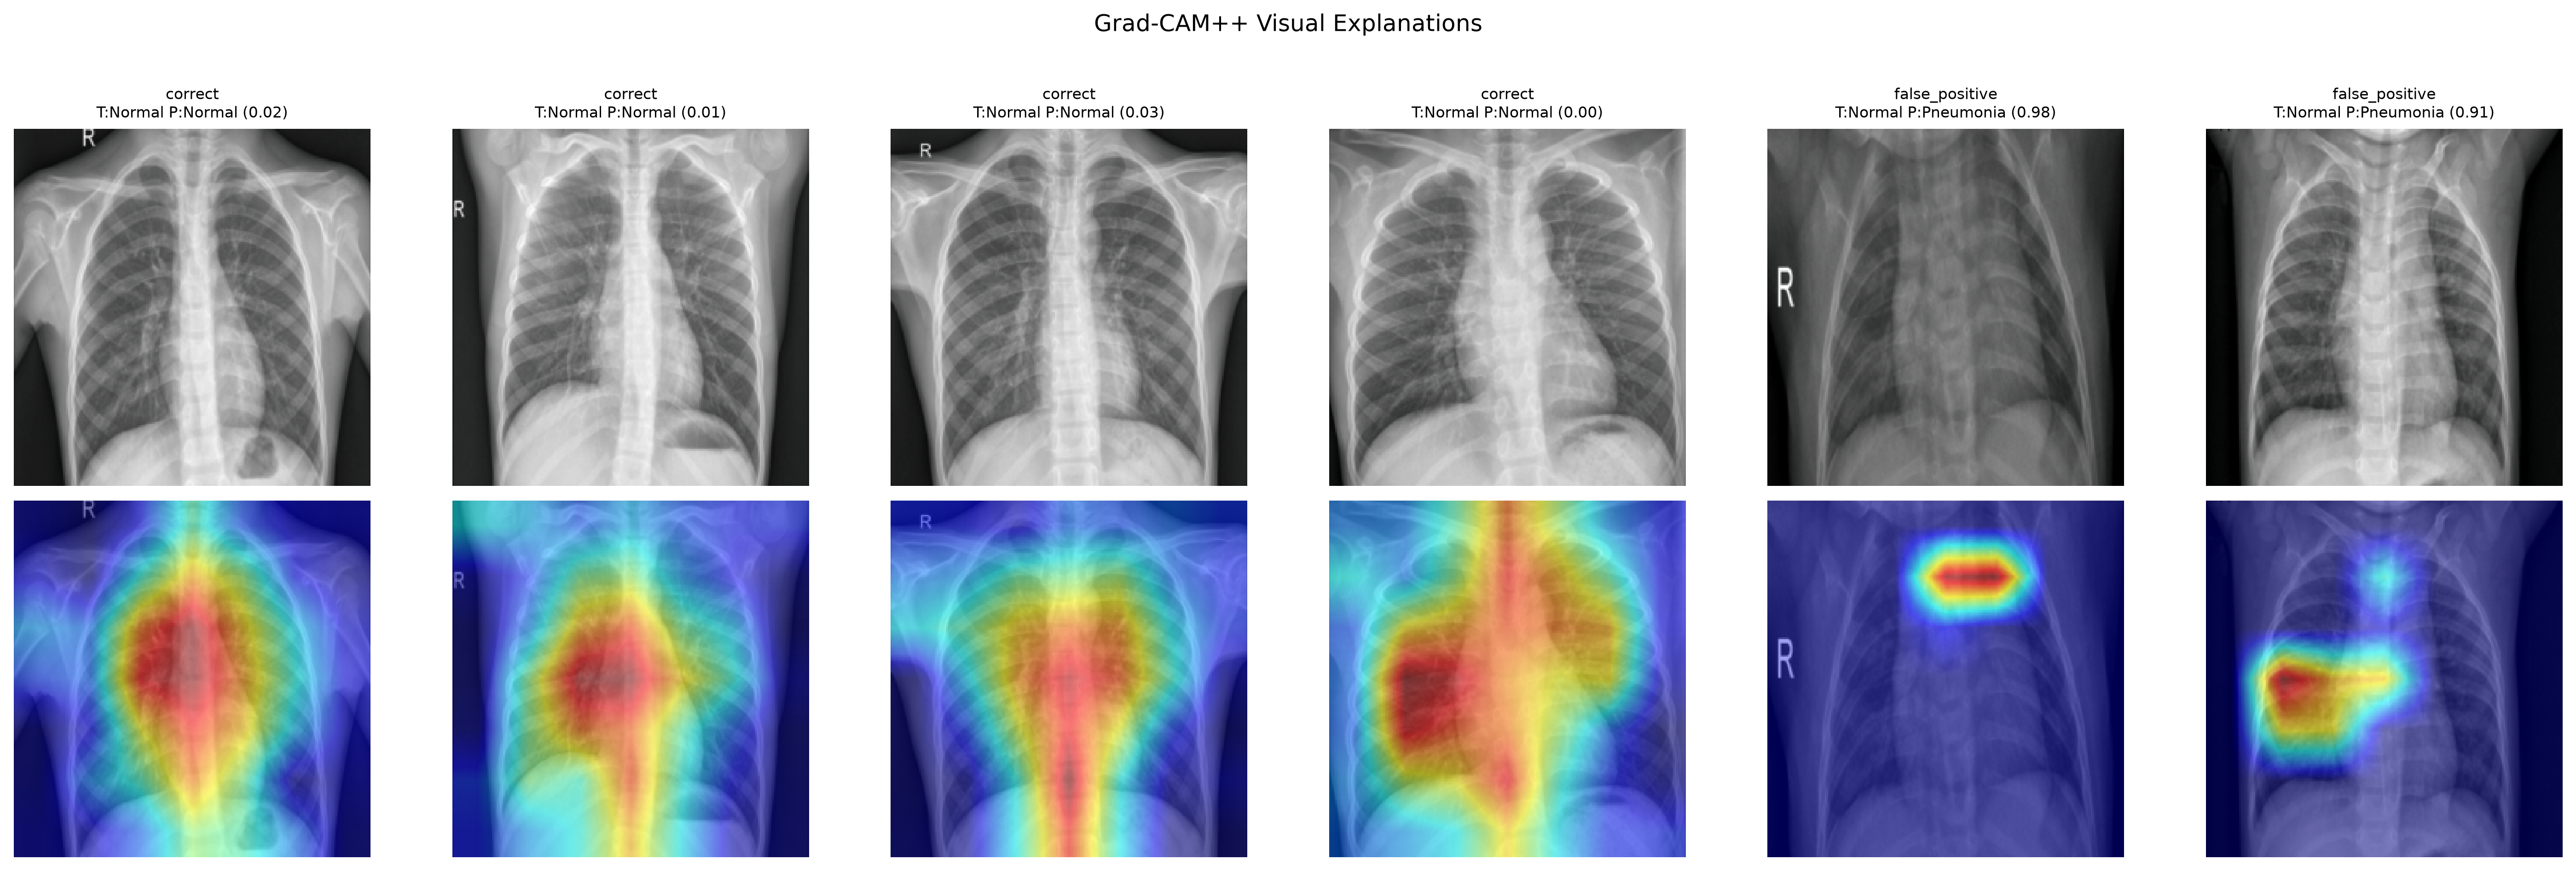
\includegraphics[width=\columnwidth]{efficientnet_b0_gradcam_grid.png}
  \caption{Grad-CAM++ overlays for correct, false-positive, false-negative cases.}
  \label{fig:gradcam}
\end{figure}

\section{Discussion}
[Trade-offs across the three axes; dynamic vs static PTQ finding; screening
positioning; threshold tuning.]

\section{Limitations and Future Work}
Single-dataset; no external/clinical/edge-hardware validation (none simulated);
potential dataset bias. Future: NIH ChestX-ray14, CheXpert, edge deployment,
TinyML, federated learning, multi-disease.

\section{Conclusion}
[Restate measured headline outcomes and the reproducibility contribution.]

\begin{thebibliography}{1}
\bibitem{rajpurkar2017} P. Rajpurkar \emph{et al.}, ``CheXNet,'' arXiv:1711.05225, 2017.
\bibitem{tan2019} M. Tan and Q. Le, ``EfficientNet,'' ICML, 2019.
\bibitem{chattopadhay2018} A. Chattopadhay \emph{et al.}, ``Grad-CAM++,'' WACV, 2018.
\bibitem{kermany2018} D. S. Kermany \emph{et al.}, ``Identifying Medical Diagnoses\ldots,'' Cell, 2018.
\end{thebibliography}

\end{document}
